\subsection*{Classification Results}
The prediction accuracy for each model by genre, and each model across all books, both before and after feature reduction are shown in Table~\ref{tab:results by genre} and Table~\ref{tab:results all}, respectively\footnote{All WordNet to Roget models are mapped from WordNet\textsuperscript{R}}.
As illustrated in both settings, the performance of nearly every model improved after we reduced the features with WordNet showing the largest improvement of an average of 11.9\% when reduced by genre and 8.8\% when reduced independent of genre.

The best performing models are indicated in bold in Table~\ref{tab:results by genre} and Table~\ref{tab:results all}.
When predicting novel success by genre, WordNet\textsuperscript{R} and WNRC\textsuperscript{R} show the best results with both models predicting a book's success class at 95.4\%.
WordNet\textsuperscript{R} is most accurate with \textsc{Adventure} books, with an accuracy of 98.5\%, while WNRC\textsuperscript{R} is able to predict the success of \textsc{Historical Fiction} books with 100\% accuracy.
When predicting the success of a book independent of genre, WordNet\textsuperscript{R} remains the most accurate at 86.3\%.

Figure~\ref{fig:wn feature reduction} illustrates the pattern of performance improvement that each model exhibits through the feature reduction process both by genre and independent of genre.
As the number of features is reduced, the average accuracy for success prediction increases until the algorithm finds the best set of features and achieves peak performance.
Then accuracy sharply drops as the feature set is reduced further.
The fact that each model demonstrates such behavior validates the effectiveness of our feature reduction method.

\begin{table}[!t]
    \caption{Accuracy (\%) of classification results for all books, before/after feature reduction}
    \label{tab:results all}
    \begin{tabular}{c|c|c}
        % \hline
        \centering
        \textsc{Model} & \textsc{Accuracy} & \textsc{Accuracy\textsuperscript{R}} \\
        \hline
        Unigram & 68.7 & \textbf{70.3} \\
        % Unigram\textsuperscript{R} & 86.2}\\
        % \hline
        % Bigram & & & & & & & & & & & & & \\
        % Bigram\textsuperscript{R} & & & & & & & & & & & & & \\
        \hline
        POS & 67.4%42330 
        & 67.4%42332 \\
        \\
        % POS\textsuperscript{R} & 73.0} \\
        \hline
        Roget & 73.5 & 74.8 \\
        % Roget\textsuperscript{R} & 81.8} \\
        \hline
        WordNet & 74.9 & \textbf{86.3} \\
        % WordNet\textsuperscript{R} & 92.6} \\
        \hline
        WNRC & 76.4 & \textbf{77.4} \\
        \hline
        WNRT & 69.5 & 69.5 \\
        % \hline
        % \hline
        % Average & ? & ?} \\
        % Average\textsuperscript{R} & 83.4} \\
        % \hline
        % $\Gamma$ & & & & & & & & & & & & & \\
        % $\Gamma^R$ & & & & & & & & & & & & & \\
        % \hline
        % $\Gamma^G$ & & & & & & & & & & & & & \\
        % $\Gamma^{G^R}$ & & & & & & & & & & & & & \\
        % \hline
        % $\gamma$ & & & & & & & & & & & & & \\
        % $\gamma^R$ & & & & & & & & & & & & & \\
        % \hline
        % $\gamma^G$ & & & & & & & & & & & & & \\
        % $\gamma^{G^R}$ & & & & & & & & & & & & & \\
        \hline
    \end{tabular}
\end{table}

\subsection*{Interpreting Book Success}\label{subsec:int book success}
While our reduced WordNet model displays excellent performance in both test settings (by genre and independent of genre), the resulting feature sets are not self-explanatory.
In other words, the Synsets that the model deems most important do not necessarily highlight some interesting aspect of successful books, expected or otherwise.
This is where \textit{Roget's Thesaurus} proves most valuable.

We figured that if we looked up the Roget Theme of each WordNet Synset that we would find that the successful and unsuccessful books prioritize different Themes.
This was possible due to the similarity in the structure of WordNet and \textit{Roget's Thesaurus} as explained in the \textbf{Methodology} section above.
With this hypothesis in mind, we mapped the reduced WordNet model to a new Roget model by first looking up the Roget Category of each Synset from the reduced WordNet feature set, and then summing the frequencies in each group of Sysnets.
Then, as we did with each previous model, we reduced the new WordNet-to-Roget-Category (WNRC) model.
From the WNRC\textsuperscript{R} model we mapped again, this time from Roget Categories to the 23 Roget Themes, which produced the WordNet-to-Roget-Themes (WNRT) model.

We did not expect the performance of the WNRC model, since it was conceived strictly as an intermediary map between WordNet and Roget Themes. 
WNRC produced the highest baseline results of all the models used in our experiments with 89.5\% average accuracy by genre, and was able to perfectly predict the success classification of \textsc{Historical Fiction} novels.
Furthermore, WNRC\textsuperscript{R} accurately predicts success classification per genre at an average rate of 95.4\%, tying it with WordNet\textsuperscript{R} as the best performing models we tested.
What's impressive about the accuracy of WNRC\textsuperscript{R} when compared to that of WordNet\textsuperscript{R} is the large difference in number of features used in each model as shown in Table~\ref{tab:wn vs wnrc features}.

\begin{table}[t]
    \caption{Number of features before/after reduction for WordNet, WNRC, and WNRT}
    \label{tab:wn vs wnrc features}
    \begin{tabular}{l|r|r|r}
        % \hline
        % \multirow{2}{*}{Genre} & \multicolumn{3}{|c}{Number of Features} \\
        % \cline{2-4}
        % & WordNet & WNRC & WNRS \\
        % \hline
        %%
        %%%%
        % UPDATE ALL %%%
        %%%%
        \centering
        \textsc{Genre} & \textsc{WordNet} & \textsc{WNRC} & \textsc{WNRT} \\
        \hline
        Adventure & 36,390 & 425 & 22 \\
        Adventure\textsuperscript{R} & 540 & 149 & 17 \\
        \hline
        Children & 39,179 & 864 & 23 \\
        Children\textsuperscript{R} & 2,117 & 210 & 14 \\
        \hline
        Detective & 31,833 & 840 & 21 \\
        Detective\textsuperscript{R} & 1,670 & 272 & 9 \\
        \hline
        Drama & 33,718 & 812 & 23 \\
        Drama\textsuperscript{R} & 1,996 & 333 & 3 \\
        \hline
        Fantasy & 32,483 & 779 & 21 \\
        Fantasy\textsuperscript{R} & 1,665 & 192 & 12 \\
        \hline
        Fiction & 43,655 & 963 & 23 \\
        Fiction\textsuperscript{R} & 4,407 & 403 & 10 \\
        \hline
        Hist. Fict. & 36,902 & 815 & 22 \\
        Hist. Fict.\textsuperscript{R} & 864 & 198 & 14 \\
        \hline
        Humor & 37,457 & 822 & 22 \\
        Humor\textsuperscript{R} & 1,493 & 324 & 7 \\
        \hline
        Poetry & 38,412 & 872 & 23 \\
        Poetry\textsuperscript{R} & 3,004 & 243 & 7 \\
        \hline
        Romance & 36,137 & 451 & 23 \\
        Romance\textsuperscript{R} & 688 & 129 & 12 \\
        \hline
        Sci-Fi & 37,835 & 617 & 23 \\
        Sci-Fi\textsuperscript{R} & 1,190 & 225 & 6 \\
        \hline
        Short & 36,912 & 964 & 22 \\
        Short\textsuperscript{R} & 3,769 & 217 & 16 \\
        \hline
        All & 48,461 & 1,001 & 23 \\
        All\textsuperscript{R} & 7,415 & 374 & 23 \\
        \hline
    \end{tabular}
\end{table}

With such impressive results from WNRC\textsuperscript{R}, we expected WNRT and WNRT\textsuperscript{R} to follow suit despite learning with a feature set of at most 23 features.
WNRT\textsuperscript{R} achieves an average accuracy of 83.7\% learning from an average of only 10 features. 
While the performance of WNRT\textsuperscript{R} is impressive given the few number of features it requires, the purpose of WNRT\textsuperscript{R} was not to outperform WordNet\textsuperscript{R} or WNRC\textsuperscript{R}.
As previously state, the motivation for the construction of WNRT was strictly to find a common thread between successful novels in each genre.
That said, the decent performance of the WNRT\textsuperscript{R} model does support the reasoning behind its conception, and provide further evidence that WordNet\textsuperscript{R} and WNRC\textsuperscript{R} are general models that can reveal underlying characteristics of successful books.

\begin{table*}[!t]
    \caption{Top 5 most important themes for classifying \textsc{Children} novels and successful/unsuccessful thematic words}
    \label{tab:child themes}
    \begin{tabular}{l|ll}
        \hline
        \centering
        \multirow{2}{*}{\textsc{Theme}} & \multicolumn{2}{c}{\textsc{Words}} \\
        \cline{2-3}
        & \multicolumn{1}{c|}{Successful} & \multicolumn{1}{c}{Unsuccessful} \\
        \hline
        Affections & enthusiastic, lively, tenderness & inactive, sluggish, dull \\
        Communication of Ideas & secret, untruth, language & school, grammar, taciturnity \\
        Formation of Ideas & incredulity, impossibility, curiosity & dissent, sanity, memory \\
        Moral & gluttony, impurity, selfishness & punishment, virtue, duty \\
        Personal & expecting, blemish, hopelessness & aggravation, dejection, dullness \\
        \hline
    \end{tabular}
\end{table*}

Additionally, WNRT does not improve performance after feature reduction when classifying independent of genre.
This outcome also supports our original hypothesis as it shows that the model requires each of the 23 Roget Themes in order to make the most accurate prediction.
The lack of improvement in WNRT\textsuperscript{R} when predicting success class independent of genre also demonstrates the relationship between a novel's genre and its prioritization of certain Themes.

\subsection*{Successful Lexical Choices}\label{subsec:successful lexical choices}

After mapping the resulting feature weights of our WordNet\textsuperscript{R} model to Roget Themes, we were able to highlight the most important Themes when classifying the success of a novel given its genre.
Table~\ref{tab:child themes} gives the most important themes in predicting the success of \textsc{Children's} novels and the successful and unsuccessful semantic word groups within those themes.
These results clearly identify words associated with "school" and "grammar" as key contributors to unsuccessful \textsc{Children's} novels, while words like "secret," "enthusiastic," and "selfishness" contribute to successful \textsc{Children's} novels.

The indicated Themes align with intuitive expectations for \textsc{Children's} books, especially the presence of \textsc{Formation of Ideas} and \textsc{Moral}.
To verify these results, we looked at the most downloaded \textsc{Children's} book, \textit{Little Women}.
We ranked each book in the \textsc{Children's} genre according to the frequency of each prioritized Themes listed in Table~\ref{tab:little women}.
Then, we looked to see where \textit{Little Women} ranked for each of the Themes.
\textit{Little Women}'s use of the top Themes matches up as expected, as it ranks in the top three for four of the five most important Themes, and eighth for the fifth as shown in Table~\ref{tab:little women}.
The opposite is true for the least downloaded books, which all rank at the bottom for use of the most important Themes.

% \begin{figure}[t]
    \centering
    \caption{\textit{Little Women} by Louisa May Alcott}
    \label{fig:little women cover}
    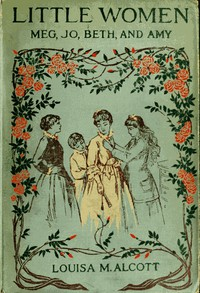
\includegraphics[width=0.25\columnwidth]{figures/pngs/little women cover.jpg}
\end{figure}

\begin{table}[h]
    \caption{Ranking the use of the most important \textsc{Children's} themes for \#1 downloaded \textsc{Children's} book, \textit{Little Women} relative to other \textsc{Children's} books in the dataset}
    \label{tab:little women}
    \begin{tabular}{l|r}
        \hline
        \centering
        \textsc{Theme} & \textsc{Rank} \\
        \hline
        Communication of Ideas & 2 \\
        Formation of Ideas & 2 \\
        Personal & 2 \\
        Moral & 3 \\
        Affections & 8 \\
        \hline
    \end{tabular}
\end{table}

Our Thematic observations hold true for each genre, but there is not one theme shared by all 12 genres.%, and Table~\ref{tab:theme counts} shows the distribution of Theme prioritization across all 12 genres.
This adheres to the observation we made about the WNRT and its lack of improvement after feature reduction for predicting success of all books.